%%%%%%%%%%%%%%%%%%%%%%%%%%%%%%%%%%%%%%%%%%%%%%%%%%%%%%%%%%%%%
%% Isolated DC-DC converters %%
%%%%%%%%%%%%%%%%%%%%%%%%%%%%%%%%%%%%%%%%%%%%%%%%%%%%%%%%%%%%%
\section{Isolated DC-DC converters}

%%%%%%%%%%%%%%%%%%%%%%%%%%%%%%%%%%%%%%%%%%%%%%%%%%%%%%%%%%%%%
%% Some fundamentals %%
%%%%%%%%%%%%%%%%%%%%%%%%%%%%%%%%%%%%%%%%%%%%%%%%%%%%%%%%%%%%%
\subsection{Some fundamentals}

%%%%%%%%%%%%%%%%%%%%%%%%%%%%%%%%%%%%%%%%%%%%%%%%%%%%%%%%%%%%%
%% Galvanic isolation %%
%%%%%%%%%%%%%%%%%%%%%%%%%%%%%%%%%%%%%%%%%%%%%%%%%%%%%%%%%%%%%
\begin{frame}
    \frametitle{Galvanic isolation}
    \begin{columns}
        \begin{column}{0.5\textwidth}
             \begin{varblock}{A definition}
                Galvanic isolation is a principle of isolating functional sections of electrical circuits to prevent a direct current flow from input to output, that is, enabling different ground potentials for the circuit sections.   
             \end{varblock}%
             \vspace{1em}
        Typical reasons for requiring galvanic isolation are:
        \begin{itemize}
            \item Safety (prevention of electric shock),
            \item Noise reduction,
            \item contact corrosion reduction.
        \end{itemize}
        \end{column}
        \begin{column}{0.5\textwidth}
            \vspace{-0.75cm}
            \begin{figure}
                \begin{subfigure}{\textwidth} 
                    \begin{circuitikz}
                        \ctikzset{blocks/scale=2, block lateral anchors pos=0.7}
                        \path (0,0) node[sdcdcshape, anchor=dc down in](dcdc){} ; 
                        \draw (dcdc.left up) -- ++(-1,0) coordinate (A1) 
                        (dcdc.left down) to [short, -*] ++(-1,0) coordinate (A2)
                        (A1) to [V, v_=$u_1$] (A2)
                        (dcdc.right up) to [short, -o]  ++(1,0) coordinate (B1)
                        (dcdc.right down) to [short, -o] ++(1,0) coordinate (B2);
                        \draw (B1) to [open, v^=$u_2$, voltage = straight] (B2);
                        \path (4,0.25) node[graduate,mirrored,sword,minimum size=1.5cm, stripes = uniblue] (human){};
                        \draw (human.south) node[ground](G2){}
                        let \p1 = (G2), \p2 = (A2) in (\x2, \y1) node[ground](G1){}
                        (G1) -- (A2);
                        \draw let \p1 = (G2), \p2 = (A2)  in (\x2, \y1) [signalred, ultra thick, -latex, dashed] (G1.south) -- (\x2,\y2) -- (\x1,\y2) -- (G2.south) -- (G1.south);
                        \draw let \p1 = (G2), \p2 = (A2)  in (\x2/2+\x1/2, \y1) node[signalred, below] {current through ground};
                    \end{circuitikz}
                \caption{Lack of galvanic isolation}
            \end{subfigure}
            \begin{subfigure}{\textwidth} 
                \begin{circuitikz}
                    \ctikzset{blocks/scale=2, block lateral anchors pos=0.7}
                    \path (0,0) node[sdcdcshape, anchor=dc down in](dcdc){} ; 
                    \draw (dcdc.left up) -- ++(-1,0) coordinate (A1) 
                    (dcdc.left down) to [short, -*] ++(-1,0) coordinate (A2)
                    (A1) to [V, v_=$u_1$] (A2)
                    (dcdc.right up) to ++(0.15,0) node[transformer, anchor=A1, scale=0.655](T){}
                    (T.A2) -- (dcdc.right down)
                    (T.B1) to [open, v^=$u_2$, voltage = straight, o-o] (T.B2);
                    \path (4.5,0.25) node[graduate,mirrored,sword,minimum size=1.5cm, stripes = uniblue] (human){};
                    \draw (human.south) node[ground](G2){}
                    let \p1 = (G2), \p2 = (A2) in (\x2, \y1) node[ground](G1){}
                    (G1) -- (A2);
                    \draw [signalgreen, ultra thick, latex-latex, dashed] (G1.south) (G2.south) -- (G1.south);
                    \draw let \p1 = (G2), \p2 = (A2)  in (\x2/2+\x1/2, \y1) node[signalgreen, below] {output $u_2$ can 'float'};
                \end{circuitikz}
                \caption{Galvanic isolation via inductive separation}
            \end{subfigure}
                \caption{Why galvanic isolation can be useful}
                \label{fig:galvanic-isolation}
            \end{figure}
        \end{column}
    \end{columns}
\end{frame}

%%%%%%%%%%%%%%%%%%%%%%%%%%%%%%%%%%%%%%%%%%%%%%%%%%%%%%%%%%%%%
%% Galvanic isolation: technical realization %%
%%%%%%%%%%%%%%%%%%%%%%%%%%%%%%%%%%%%%%%%%%%%%%%%%%%%%%%%%%%%%
\begin{frame}
    \frametitle{Galvanic isolation: technical realization}
    \begin{table}
		\centering
		\begin{tabular}{M{0.3\textwidth} M{0.3\textwidth} M{0.3\textwidth}}
			\onslide<1->{Capacative} & \onslide<2->{Optical} & \onslide<3->{Inductive}\\[1em]

			\onslide<1->{
			\begin{circuitikz}
				\draw (0,-0.5) to [capacitor] (2,-0.5)
                (0,0.5) to [capacitor] (2,0.5);
			\end{circuitikz}
			}

			&
			\onslide<2->{
			\begin{circuitikz}
				\draw (0,0.5) to [empty photodiode, mirror] (2,0.5)
                (0,-0.5) to [empty led] (2,-0.5);
			\end{circuitikz}
			}
			
			&
			\onslide<3->{
			\begin{circuitikz}
				\draw (0,0) node[transformer](){};
			\end{circuitikz}
			}
            
            \\[1em]  
            
            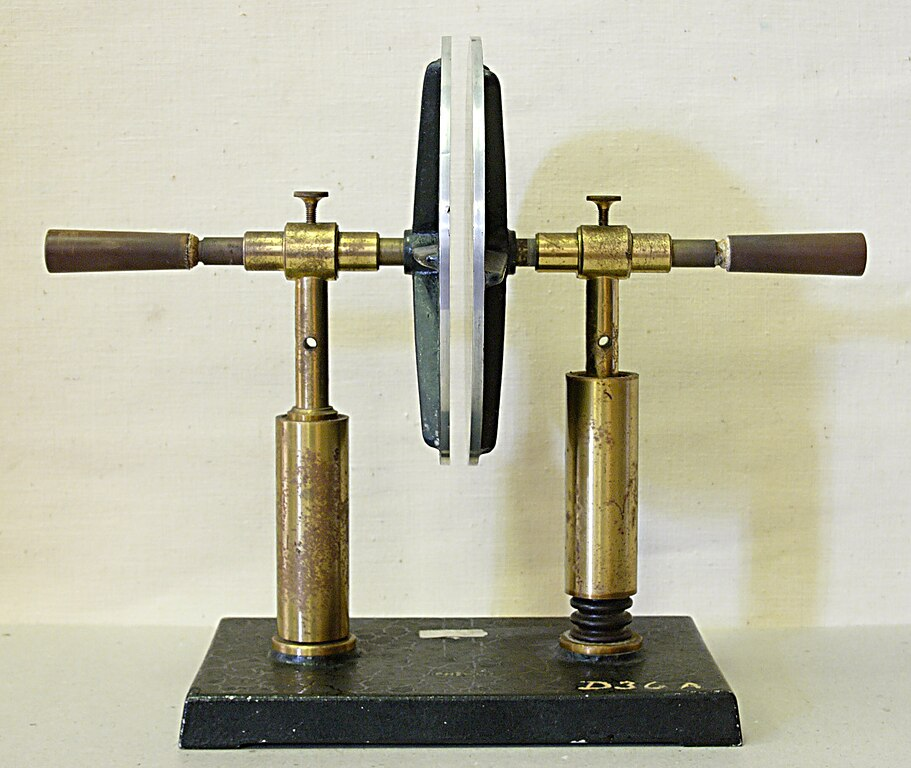
\includegraphics[height=0.25\textheight]{fig/lec03/Capacitor_example.jpg}
            
            {\small source: \href{https://commons.wikimedia.org/wiki/File:Plattenkondensator_hg.jpg}{Wikimedia Commons}, H.~Grobe, \href{https://creativecommons.org/licenses/by/3.0/deed.en}{CC~BY~3.0}}

            &

            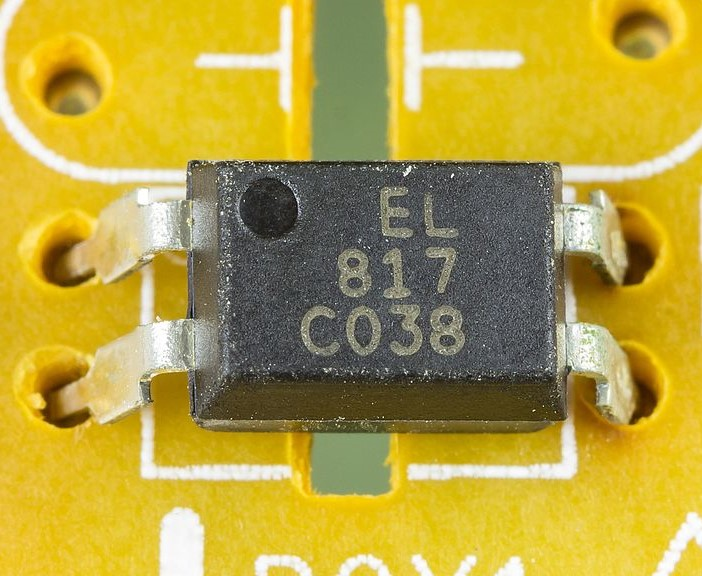
\includegraphics[height=0.25\textheight]{fig/lec03/Optocoupler_example.jpg}

            {\small source: \href{https://en.wikipedia.org/wiki/File:Philips_BDP3280-12_-_Everlight_EL817_on_power_board-1779.jpg}{Wikimedia Commons}, R.~Spekking, \href{https://creativecommons.org/licenses/by-sa/4.0/deed.en}{CC~BY-SA~4.0}}

            &
            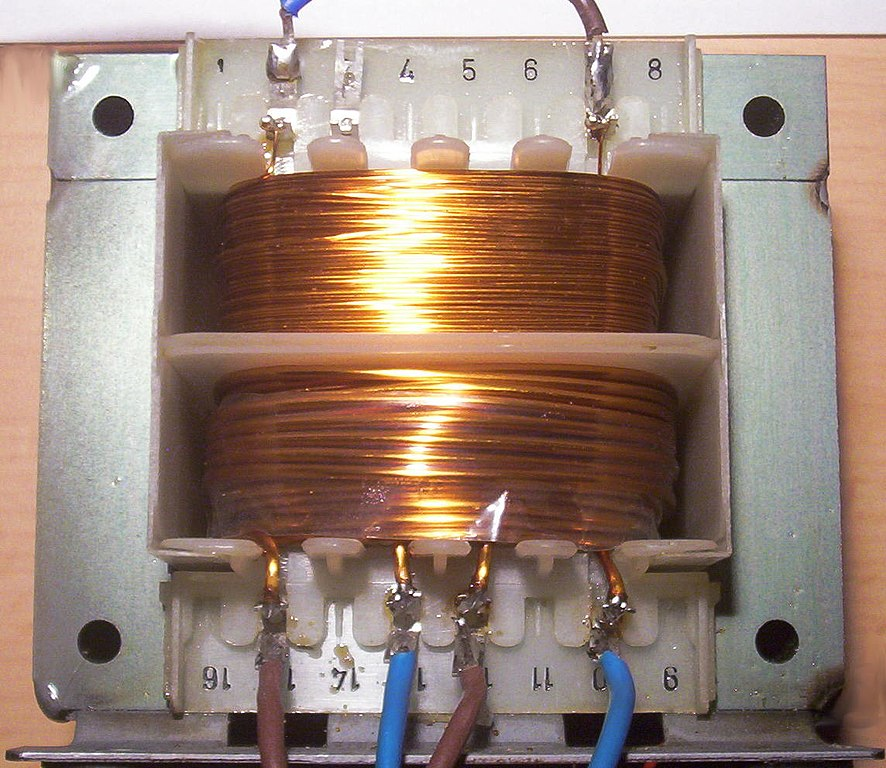
\includegraphics[height=0.25\textheight]{fig/lec03/Transformer_example.jpg}

            {\small source: \href{https://commons.wikimedia.org/wiki/File:Trafo-innenleben.jpg}{Wikimedia Commons}, S.~Riepl, public domain}


		\end{tabular}
	\end{table}
\end{frame}


%%%%%%%%%%%%%%%%%%%%%%%%%%%%%%%%%%%%%%%%%%%%%%%%%%%%%%%%%%%%%
%% Flyback converter %%
%%%%%%%%%%%%%%%%%%%%%%%%%%%%%%%%%%%%%%%%%%%%%%%%%%%%%%%%%%%%%
\subsection{Flyback converter}

%%%%%%%%%%%%%%%%%%%%%%%%%%%%%%%%%%%%%%%%%%%%%%%%%%%%%%%%%%%%%
%% Forward converter %%
%%%%%%%%%%%%%%%%%%%%%%%%%%%%%%%%%%%%%%%%%%%%%%%%%%%%%%%%%%%%%
\subsection{Forward converter}